%%%%%%%%%%%%%%%%%%%%%%%%%%%%%%%%%%%%%%%%%%%%%%%%%%%%%%%%%%%%%%%%%
\chapter{FUTURE WORK}\label{ch:ch7}
%%%%%%%%%%%%%%%%%%%%%%%%%%%%%%%%%%%%%%%%%%%%%%%%%%%%%%%%%%%%%%%%%

Extracting the essence of nature's working principles has always attracted curious minds. Biomimetics or biomimicry is becoming a more appreciated source of inspiration for system designs in a variety of topics, thanks to the rapid development of technology enabling to reveal the mysterious mechanisms evolved in centuries by nature. Utilization of these uncovered working principles on science and engineering problems offer elegant solutions for challenges. 

The idea of impedance pump is inherited from the developmental biology of the embryonic vertebrate heart. The researchers have been amazed realizing that blood pumping in the embryonic vertebrate heart starts before the the discernable chambers and valves have been developed. Although this phenomenon has been explained as peristaltic motion in early stages, advances in confocal laser scanning microscopy and four-dimensional visualization, utilized to investigate the cell movements of embryonic zebrafish hearth tube, showed contradictory foundings \cite{forouhar2006embryonic}. Forouhar and his colleagues offered that this can be explained with the elastic wave propagation in the heart tube causing a suction induces that pumping behavior. 

It is comprised of flexible tubing of different impedances filled with fluid. The advantage is that a flow can be induced without the need for valves but by applying a compression at asymmetric positions from the ends. The frequency of the pinching has a major importance on the flow characteristics and the direction of the flow can even be reversed by changing the frequency and duty cycle. 

The study of valveless pumps goes back to 1954 when Gerhart Libeau got suspicious about the high efficiency of blood circulations may not be explained only by the work done by the heart \cite{LiebauStartedThis,Liebau2,Liebau3}. 
 Although he also achieved to show through experiments that the valveless pumping (See Fig. ~\ref{fig:liebau}) effect in elastic tubes exists, an attempt to model the phenomenon  delayed more than 10 years until von Bredow \cite{firstCompWork} derived a set of linear equations matcing Liebau phenomenon. Consideringring an elastic tube connecting two tanks, Rath and Teipel \cite{CompWorkRathTeipel} developed a nonlinear mathematical model for this one dimensional flow problem and solved it numerically. Takagi and Takahashi \cite{rigidPipesTakagi} were the first to show experimentally and numerically that the valveless pumping is possible for rigid pipes, although previous numerical studies also indicated that result \cite{numInvLiebauPhenom}.
 
 % For one-column wide figures use
\begin{figure*}
	\centering
% Use the relevant command to insert your figure file.
% For example, with the graphicx package use
  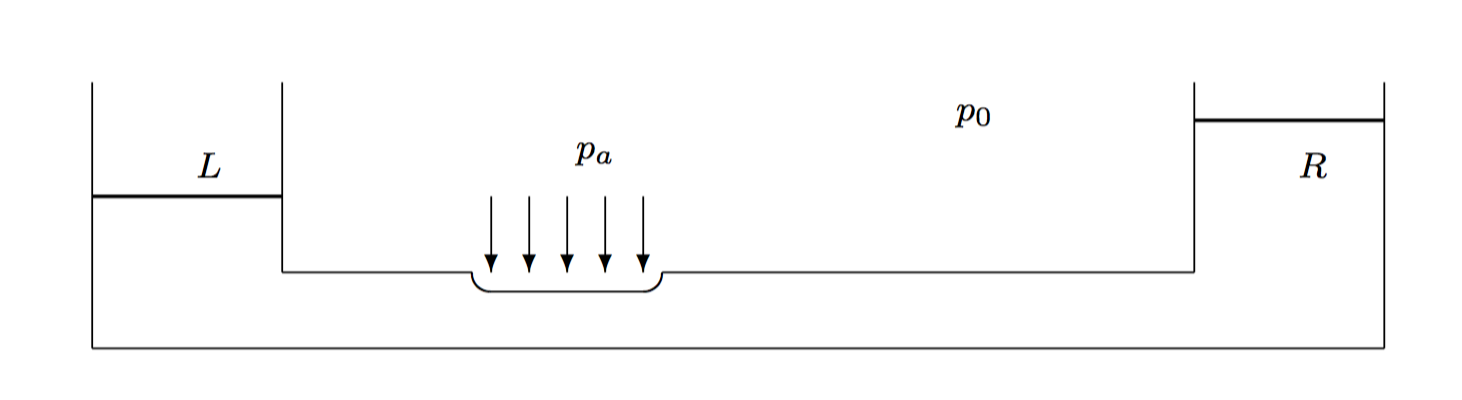
\includegraphics[scale=0.45]{figures/liebau}
% figure caption is below the figure
\vspace*{6mm}
\caption{A Liebau pump \cite{numInvLiebauPhenom}}
\label{fig:liebau}       % Give a unique label
\end{figure*}
 
 Addition of nanofluids to this pumping mechanism might lead to interesting results. Using an external magnetic field to induce motion instead of pinching might be considered. A challenge to cope with is the limited number of studies investigating numerical models for this pumping mechanism.
 